\documentclass[12pt]{article}
\usepackage{amsmath, amssymb}
\usepackage{amsthm}
\usepackage{hyperref}
\usepackage{MnSymbol}
%%\usepackage[pdftex]{graphicx}
\usepackage{enumerate}
\usepackage{amsmath}
\usepackage{amssymb}
\usepackage{multicol}
\usepackage{algpseudocode}
\usepackage{algorithm}


\usepackage[final]{graphicx}
\usepackage{subcaption}
\renewcommand{\phi}{\varphi}
\newcommand{\rarrow}{\rightarrow}
\usepackage{ listings}
\title{COMP 540: Homework 5}

\author{Guangyuan Yu(gy12) and Andrew Wells}
%Replace Partner 1 and 2 with your names.

\begin{document}
\maketitle


\section*{Solution 1}
\begin{itemize}
\item Why do deep networks typically outperform shallow networks?

We assume this question means to compare networks with a similar number of nodes to make the comparison ?fair.? So the question is why do deep networks with ~N nodes perform better than shallow but wide networks with ~N nodes. The answers in the literature generally point to the ability to learn ?more general concepts.? A shallow and wide network can ?memorize? the training data quite well but it does not have the ability to learn ?general concepts? and thus will tend to overfit the training data.\\ (http://stats.stackexchange.com/questions/222883/why-are-neural\\-networks-becoming-deeper-but-not-wider)\\ (http://jmlr.org/proceedings/papers/v33/pandey14.pdf)

\item What is leaky ReLU activation and why is it used?

A leaky ReLU is similar to the hinge function but instead of f(x) = 0 when $x < 0$ we have f(x) = 0.01x when $x < 0$. It is useful because it has similar properties to the hinge loss function (it is differentiable except at x=0) and additionally for $x < 0$ it discriminates slightly for different x, i.e. it is strictly increasing. This avoids the ?dying ReLU? problem where the weights could be set such that a unit will never activate again and there is no way for the network to tell the difference because the unit is always at 0 instead of varying slightly in small negative numbers. 

\item In one or more sentences, and using sketches as appropriate, contrast: AlexNet, VGG-Net, GoogleNet and ResNet. What is the one defining characteristic of each network?

AlexNet: 8 layers with 15.4 percent error rate.\\
layer1:con(96 channel,11*11 kernalsize,stride=4)+Relu+maxpool+LRN\\
layer2:con(256 channel,5*5kernalsize)+Relu+maxpool+LRN\\
layer3:con(384 channel)+Relu\\
layer4:con(384 channel)+Relu\\
layer5:con(256 channel)+Relu+maxpool\\
layer6:fc+relu\\
layer7:fc+relu\\
layer8:fc+relu\\
Defining feature: layer is made of convolution, Relu, Maxpool and Fully connect layer.\\





VGG-Net: 19 layers with 7.3 percent error rate. Defining feature:The net is trained layer by layer, when the previous layer is trained to be stable, then adding the next layer to the system.\\
GoogleNet: 41 layers with 6.67 percent error rate.According to the abstract: ?The main hallmark of this architecture is the improved utilization of the computing resources inside the network. This was achieved by a carefully crafted design that allows for increasing the depth and width of the network while keeping the computational budget constant.? The defining characteristic is that on one convolution layer, they use different kernalsize like 3*3 and 5*5, and combine them together as one convolution layer \\
ResNet:  152 layers with 3.6 percent error rate.The defining characteristic is that the input of some layers has a identity copy of previous layers, so the parameter is not the optimal solution, the difference is called Residual. \\

\end{itemize}

\section*{Solution 2}
\begin{itemize}
\item we start with the equation:
\begin{equation}
H(q) = -q log q - (1-q) log (1-q)
\end{equation}
When we calculate the derivative:
\begin{equation}
\frac{\partial H(q)}{q}=-log(q)-1-(1-q)*\frac{-1}{(1-q)}-(-1)log(1-q)=0
\end{equation}
and we get 
\begin{equation}
log(\frac{1-q}{q})=0
\end{equation}
when $q=0.5,H(0.5)=1$
when $q=0,H(0)=0$
when $q=1,H(1)=0$
so H(0.5)is the maximum,$H(q)<=1$\\
when =0.5 means p=n



\item
The misclassification rates are:\\
Model A: 25 percent.\\
Model B: 25 percent.\\



The original entropy is\\ -0.5log(0.5)-0.5log(0.5)=1\\
For A:\\
$E_{left}=-0.75*log(0.75)-0.25*log(0.25)=0.8113$\\
$E_{right}=-0.75*log(0.75)-0.25*log(0.25)=0.8113$\\
$E_{A}=0.5*E_{left}+0.5*E_{right}=0.8113$\\
$EGAIN=0.8113-1=-0.1887$\\
For B:\\
$E_{left}=-\frac{2}{6}*log(\frac{1}{3})-\frac{4}{6}*log(\frac{4}{6})=0.9183$\\
$E_{right}=0$\\
$E_{B}=6/8*E_{left}+2/8*E_{right}=0.6887$\\
$EGAIN=0.6887-1=-0.3113$\\
So the entropy gain is lower for B\\


For the Gini index we have:\\
For A:\\
p=0.75 for left\\
p=0.75 for right\\
giniA=2*0.75*0.25*0.5+2*0.75*0.25*0.5=3/8\\
For B:\\
p=2/3 for left\\
p=1 for right\\
giniB=2*2/3*1/3*6/8=1/3\\
$giniB<giniA$\\






\item
The misclassification rate should only decrease. Intuitively this can be seen because we can always ignore the feature (i.e., place the points in the same bucket) so we should never be forced to make worse classifications by considering a new feature in this node. However, in practice splitting too much will lead to overfitting.

\end{itemize}
\section*{Solution 3}
\begin{itemize}
\item 
From the above we have:

\begin{equation}
E_{bag} = E_X[\epsilon_{bag}(x)^2]
\end{equation}

\begin{equation}
E_{av} = \frac{1}{L}\sum_{l=1}^LE_X[\epsilon_{l}(x)^2]
\end{equation}


\begin{equation}
\epsilon_{bag}=\frac{1}{L}{\displaystyle \sum_{l=1}^{L}\epsilon_{l}(x)}
\end{equation}

\begin{equation}
\begin{split}
E_{BAG}&=E_{X}((\epsilon_{bag})^{2})\\&=E_{X}((\frac{1}{L}{\displaystyle \sum_{l=1}^{L}\epsilon_{l}(x)})^{2})\\&=\frac{1}{L^{2}}E_{X}(\epsilon_{1}(x)^{2}+\epsilon_{2}(x)^{2}+...+\epsilon_{L}(x)^{2}+2\epsilon_{1}(x)\epsilon_{2}(x)+2\epsilon_{1}(x)\epsilon_{L}(x)+...+)\\&=\frac{1}{L^{2}}E_{X}(\epsilon_{1}(x)^{2}+\epsilon_{2}(x)^{2}+...+\epsilon_{L}(x)^{2})+\frac{1}{L^{2}}E_{X}(2\epsilon_{1}(x)\epsilon_{2}(x)+2\epsilon_{1}(x)\epsilon_{L}(x)+...+)\\&=\frac{1}{L^{2}}E_{X}(\epsilon_{1}(x)^{2}+\epsilon_{2}(x)^{2}+...+\epsilon_{L}(x)^{2})\\&=\frac{1}{L^{2}}{\displaystyle \sum_{l=1}^{L}}E_{X}(\epsilon_{l}(x)^{2})=\frac{1}{L}E_{av}
\end{split}
\end{equation}




\item
from Jensen's equality

\begin{equation}
f({\displaystyle \sum_{l=1}^{L}}\lambda_{l}x_{l})\leq{\displaystyle \sum_{l=1}^{L}}\lambda_{l}f(x_{l}) 
\end{equation}
for any
\begin{equation}
\sum_{l=1}^{L}\lambda_{l}=1 
\end{equation}
let 
\begin{equation}
\lambda_{l}=1/L
\end{equation}
\begin{equation}
(\frac{1}{L}{\displaystyle \sum_{l=1}^{L}}\epsilon_{l})^{2}\leq{\displaystyle \frac{1}{L}\sum_{l=1}^{L}}(\epsilon_{l})^{2}
\end{equation}
They are all positive, so we have:
\begin{equation}
E_{X}(\frac{1}{L}{\displaystyle \sum_{l=1}^{L}}\epsilon_{l})^{2}\leq E_{X}({\displaystyle \frac{1}{L}\sum_{l=1}^{L}}(\epsilon_{l})^{2}) 
\end{equation}

This is  $E_{bag}\leq E_{av}$






\end{itemize}


\section*{4 Fullyconnected neural networks and convolutional neural network}
\subsection*{P4.1.1 Affine layer forward}
\begin{lstlisting}
  xr = x.reshape(x.shape[0], np.prod(x.shape[1:]))
  out = xr.dot(theta) + theta0
\end{lstlisting}
Testing affine\_forward function:
difference:  9.76985004799e-10



\subsection*{P4.1.2 Affine layer backward}
\begin{lstlisting}
  xr = x.reshape(x.shape[0], np.prod(x.shape[1:]))
  dx = (dout.dot(theta.T)).reshape(*x.shape)
  dtheta = xr.T.dot(dout)
  dtheta0 = np.sum(dout, axis=0)
\end{lstlisting}
Testing affine\_backward function:
dx error:  4.20165388811e-10
dtheta error:  2.32951617865e-10
dtheta0 error:  8.90638546591e-12

\subsection*{P4.1.3 ReLU layer forward}
\begin{lstlisting}
out = np.maximum(0 * x, x)
\end{lstlisting}

Testing relu\_forward function:
difference:  4.99999979802e-08

\subsection*{P4.1.4 ReLU layer backward}
\begin{lstlisting}

dx = np.where(x > 0, dout, 0)
\end{lstlisting}
Testing relu\_backward function:
dx error:  3.27563568106e-12


\subsection*{sandwich}
Testing affine\_relu\_backward:
dx error:  3.4155090119e-10
dtheta error:  1.50178377986e-10
dtheta0 error:  2.37389897738e-11

\subsection*{softmax and SVM}
Testing svm\_loss:
loss:  9.00378308366
dx error:  8.18289447289e-10

Testing softmax\_loss:
loss:  2.30296385957
dx error:  8.76423622467e-09

\subsection*{P4.1.5 Two layer network}
\begin{lstlisting}
For the __init__ function:
    self.params['theta1'] = np.random.randn(
            input_dim, hidden_dim) * weight_scale
    self.params['theta1_0'] = np.zeros((hidden_dim,))
    self.params['theta2'] = np.random.randn(
            hidden_dim, num_classes) * weight_scale
    self.params['theta2_0'] = np.zeros((num_classes,))
    
 For the loss function:      
    
        l1_out, cache1 = affine_relu_forward(
            X, self.params['theta1'], self.params['theta1_0'])
    scores, cachea2 = affine_forward(
            l1_out, self.params['theta2'], self.params['theta2_0'])
            
      
            
                loss, dx = softmax_loss(scores, y)
    loss += self.reg / 2. * (np.sum(self.params['theta1'] ** 2) + np.sum(self.params['theta2'] ** 2))

    dx2, dtheta2, dtheta_02 = affine_backward(dx, cachea2)
    grads['theta2'] = dtheta2 + self.reg * self.params['theta2']
    grads['theta2_0'] = dtheta_02

    dx, dtheta, dtheta_01 = affine_relu_backward(dx2, cache1)
    grads['theta1'] = dtheta + self.reg * self.params['theta1']
    grads['theta1_0'] = dtheta_01
\end{lstlisting}
Testing initialization ... 
Testing test-time forward pass ... 
Testing training loss (no regularization)
Running numeric gradient check with reg =  0.0
theta1 relative error: 2.13e-08
theta1\_0 relative error: 8.37e-09
theta2 relative error: 3.31e-10
theta2\_0 relative error: 2.53e-10
Running numeric gradient check with reg =  0.7
theta1 relative error: 2.53e-07
theta1\_0 relative error: 1.56e-08
theta2 relative error: 1.37e-07
theta2\_0 relative error: 9.09e-10


\subsection*{P4.1.6 overfitting a two layer network}
\begin{lstlisting}
hl = [100]

regs = [1]
for h in hl:
    for reg in regs:
        #1, 50; .3 100
        model = TwoLayerNet(hidden_dim = h,reg = reg)
        sgd_solver = solver.Solver(model, data, update_rule='sgd', optim_config={
            'learning_rate': 1e-3,}, lr_decay=0.95, num_epochs=10, batch_size=100, 
            print_every=100)
        sgd_solver.train()
\end{lstlisting}
Here is the result:
(Iteration 4501 / 4900) loss: 1.421155
(Iteration 4601 / 4900) loss: 1.401276
(Iteration 4701 / 4900) loss: 1.392804
(Iteration 4801 / 4900) loss: 1.365272
(Epoch 10 / 10) train acc: 0.506000; val\_acc: 0.507000
\begin{figure}[H]
  \caption{loss and accuracy}
  \centering
    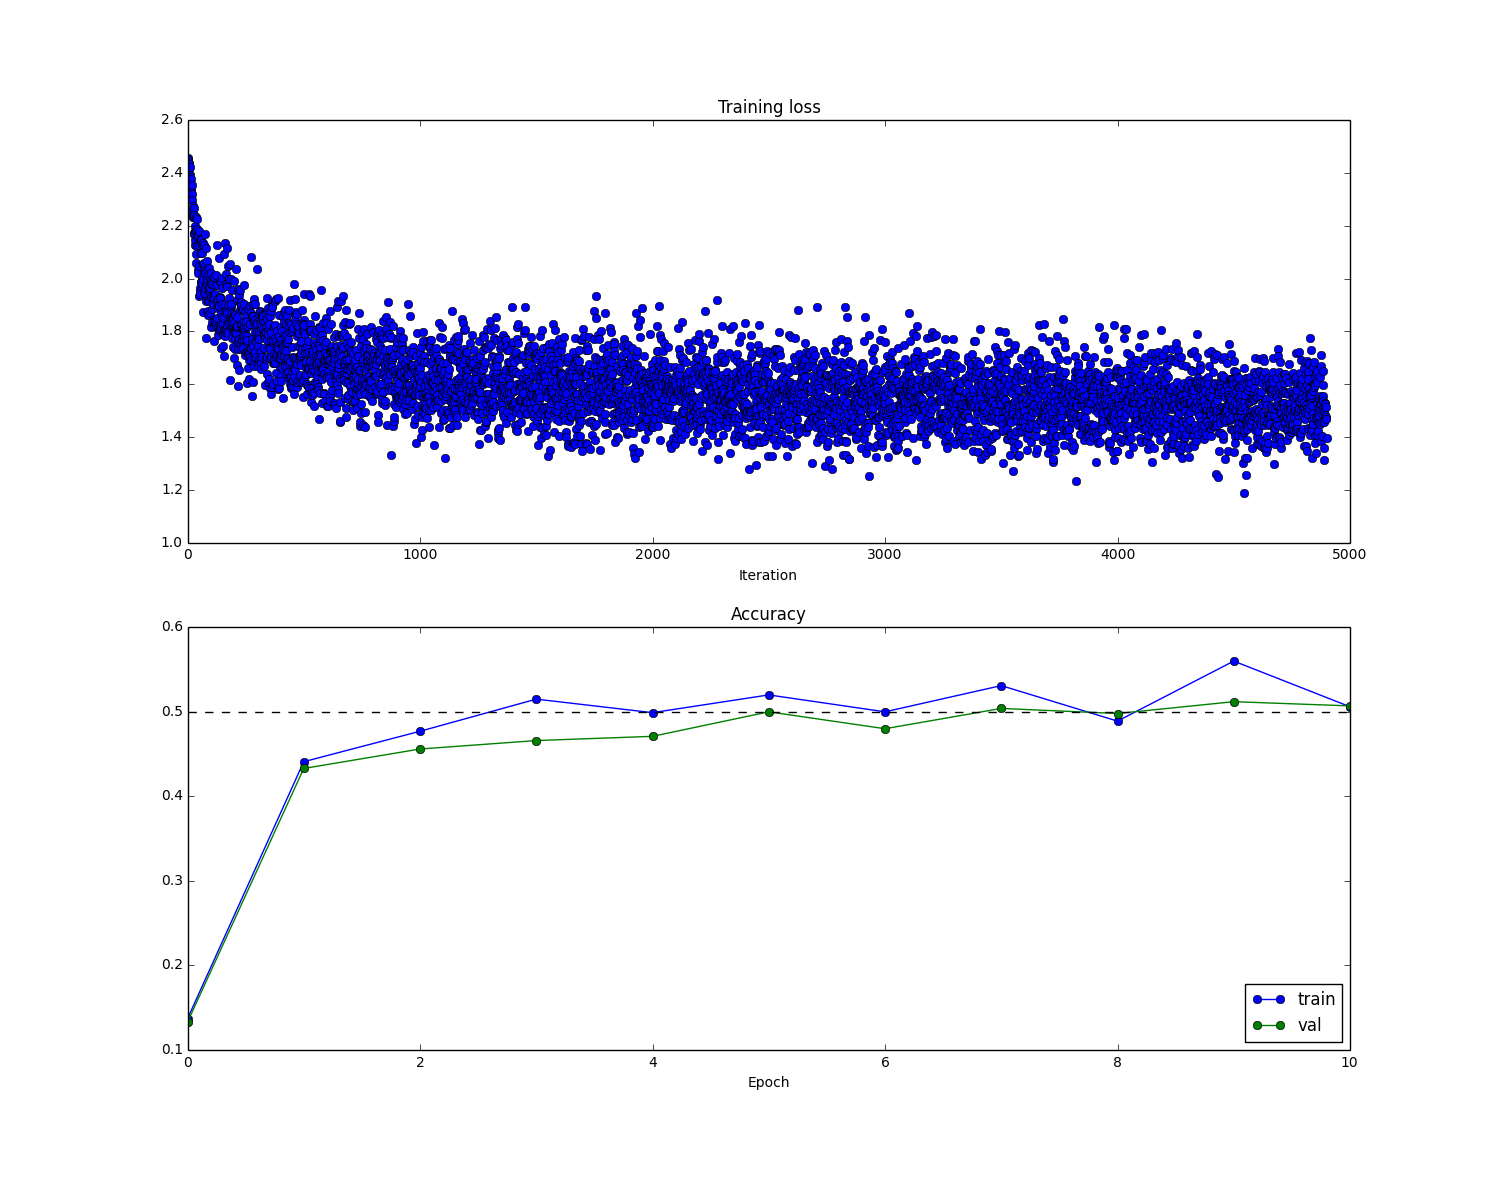
\includegraphics[scale=0.5]{lossandacc.png}
\end{figure}

\subsection*{P4.1.7 Multilayer network }
\begin{lstlisting}
For the __init__ function:
dims = [input_dim] + hidden_dims + [num_classes]
    for i in xrange(self.num_layers):
        self.params['theta' + str(i + 1)] = np.random.randn(
                dims[i], dims[i + 1]) * weight_scale
        self.params['theta' + str(i + 1) + '_0'] = np.zeros((dims[i + 1],))
 for the loss funcition:
 out = X
    caches = [0] * self.num_layers
    for i in xrange(self.num_layers - 1):
        out, caches[i] = affine_relu_forward(out, self.params['theta' + str(i + 1)],
                                                 self.params['theta' + str(i + 1) + '_0'])

    scores, caches[-1] = affine_forward(out, self.params['theta' + str(self.num_layers)],
                                            self.params['theta' + str(self.num_layers) + '_0'])
        
   loss, dx = softmax_loss(scores, y)

    dx, dtheta, dtheta_0 = affine_backward(dx, caches[-1])
    grads['theta' + str(self.num_layers)] = dtheta + \
            self.reg * self.params['theta' + str(self.num_layers)]
    grads['theta' + str(self.num_layers) + '_0'] = dtheta_0
    loss += self.reg / 2 * np.sum(self.params['theta' + str(self.num_layers)] ** 2)

    for i in xrange(self.num_layers - 1):
        theta = 'theta' + str(self.num_layers - 1 - i)
        dx, dtheta, dtheta_0 = affine_relu_backward(
                dx, caches[self.num_layers - 1 - (i + 1)])
        grads[theta] = dtheta + self.reg * self.params[theta]
        grads[theta + '_0'] = dtheta_0
        loss += self.reg / 2 * np.sum(self.params[theta] ** 2)

   
    
\end{lstlisting}

Do the initial losses seem reasonable?
Here is the result:
Running check with reg =  0
Initial loss:  2.28667430954
theta1 relative error: 1.03e-06
theta1\_0 relative error: 2.14e-08
theta2 relative error: 2.57e-07
theta2\_0 relative error: 4.71e-09
theta3 relative error: 6.17e-08
theta3\_0 relative error: 1.19e-10
Running check with reg =  3.14
Initial loss:  6.67106669744
theta1 relative error: 6.25e-08
theta1\_0 relative error: 6.59e-09
theta2 relative error: 2.32e-07
theta2\_0 relative error: 7.14e-10
theta3 relative error: 3.49e-06
theta3\_0 relative error: 1.70e-10
Yes, the initial losses look reasonable, and the relative errors of all kinds of theta are very small.

\subsection*{P4.1.8 overfitting a three layer network}
Here is the result
(Iteration 31 / 40) loss: 0.123920
(Epoch 16 / 20) train acc: 1.000000; val\_acc: 0.194000
(Epoch 17 / 20) train acc: 1.000000; val\_acc: 0.207000
(Epoch 18 / 20) train acc: 1.000000; val\_acc: 0.203000
(Epoch 19 / 20) train acc: 1.000000; val\_acc: 0.208000
(Epoch 20 / 20) train acc: 1.000000; val\_acc: 0.194000




\begin{figure}[H]
  \caption{Training loss history}
  \centering
    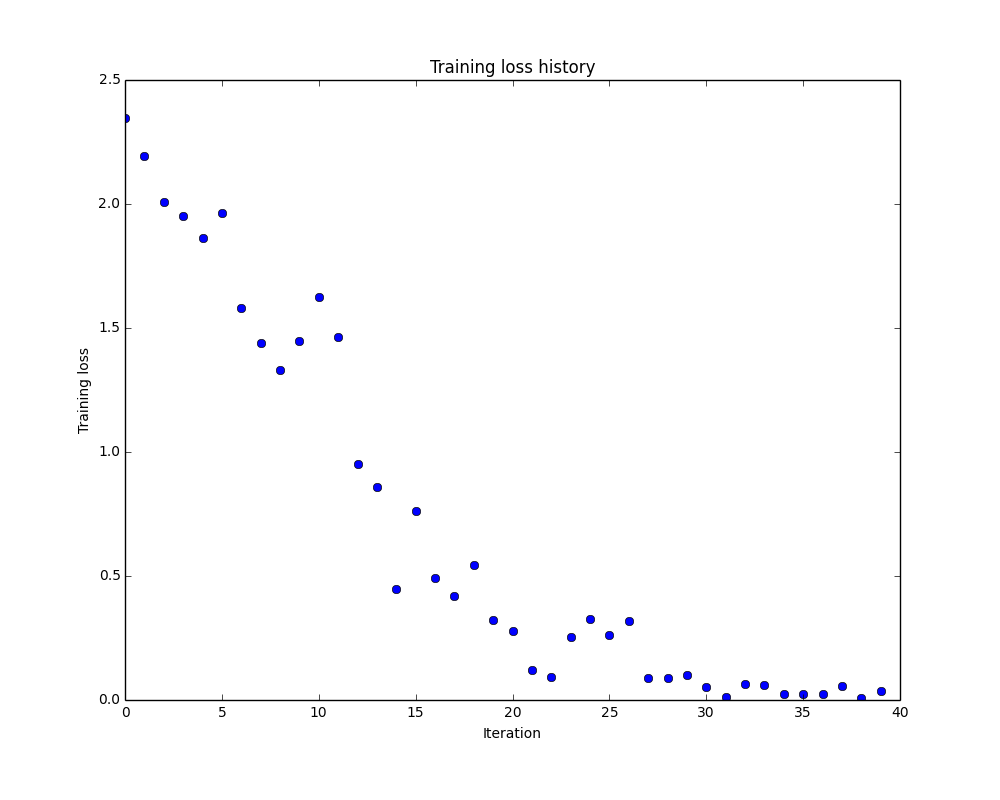
\includegraphics[scale=0.5]{mltrainingloss.png}
\end{figure}

\begin{figure}[H]
  \caption{Training loss and accuracy}
  \centering
    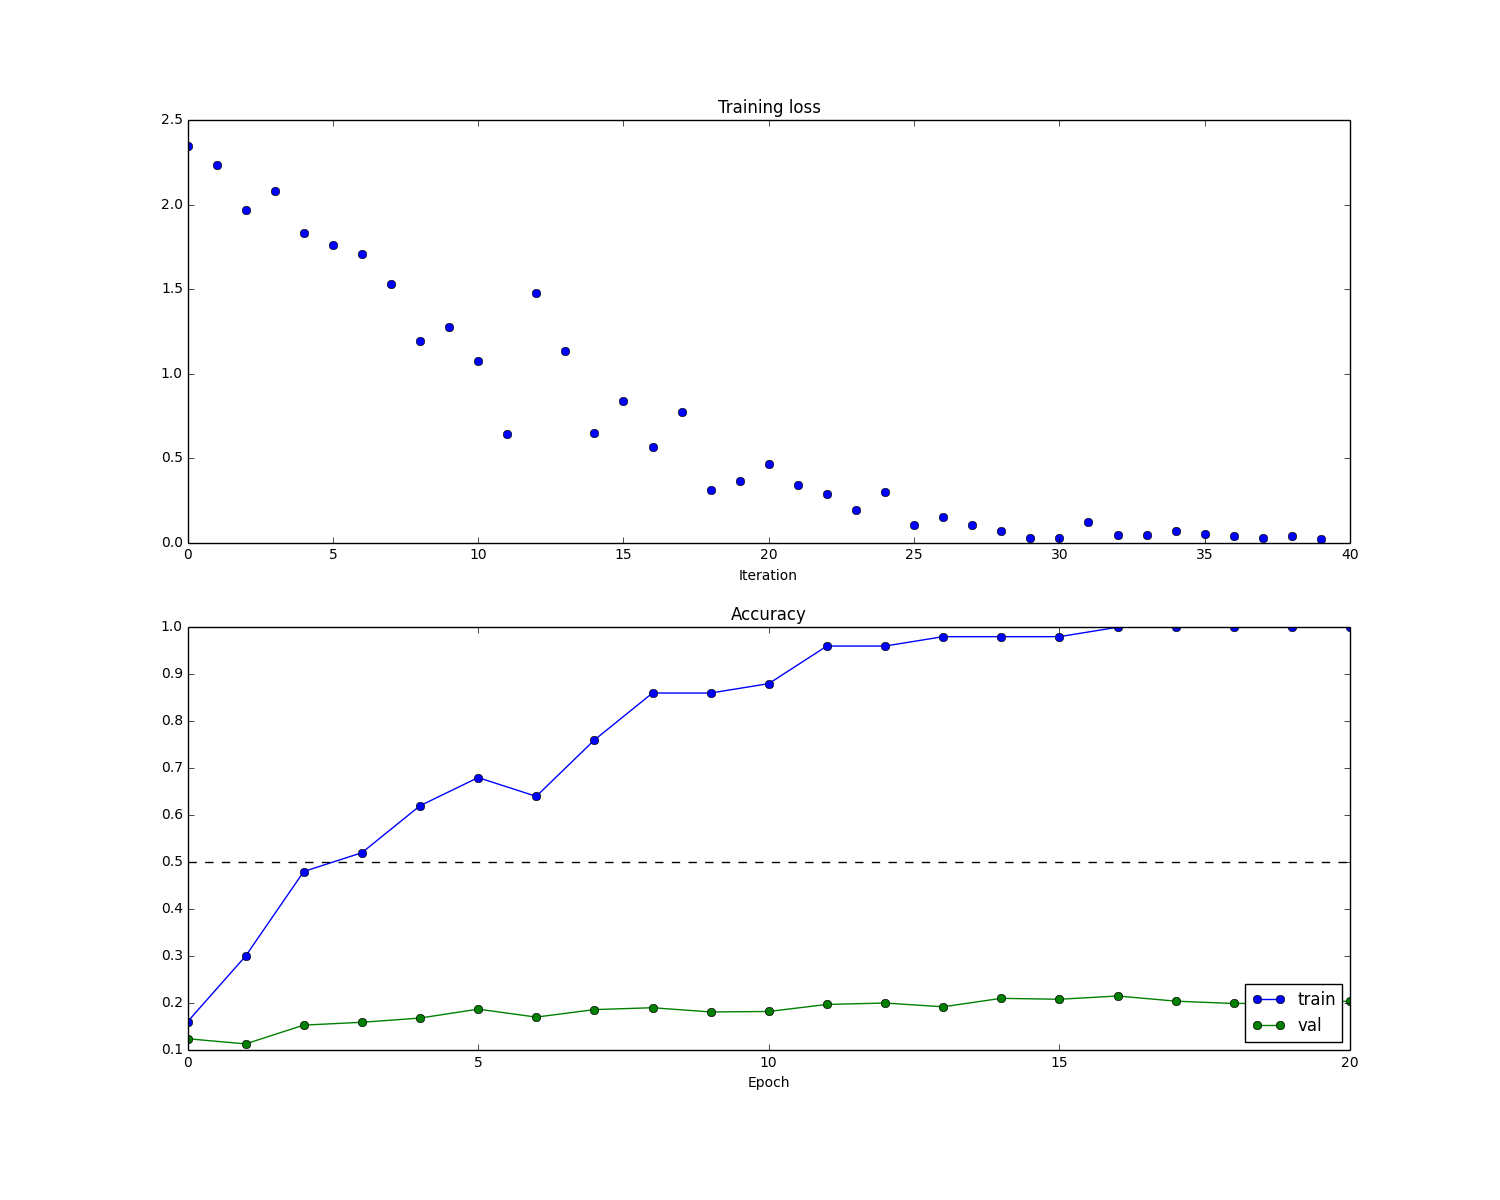
\includegraphics[scale=0.5]{mltrainingandacc.png}
\end{figure}

\subsection*{P4.1.9 overfitting a 5 layer network}
Here is the result:
(Iteration 31 / 40) loss: 0.055382
(Epoch 16 / 20) train acc: 1.000000; val\_acc: 0.155000
(Epoch 17 / 20) train acc: 1.000000; val\_acc: 0.162000
(Epoch 18 / 20) train acc: 1.000000; val\_acc: 0.164000
(Epoch 19 / 20) train acc: 1.000000; val\_acc: 0.156000
(Epoch 20 / 20) train acc: 1.000000; val\_acc: 0.164000

\begin{figure}[H]
  \caption{Training loss and accuracy}
  \centering
    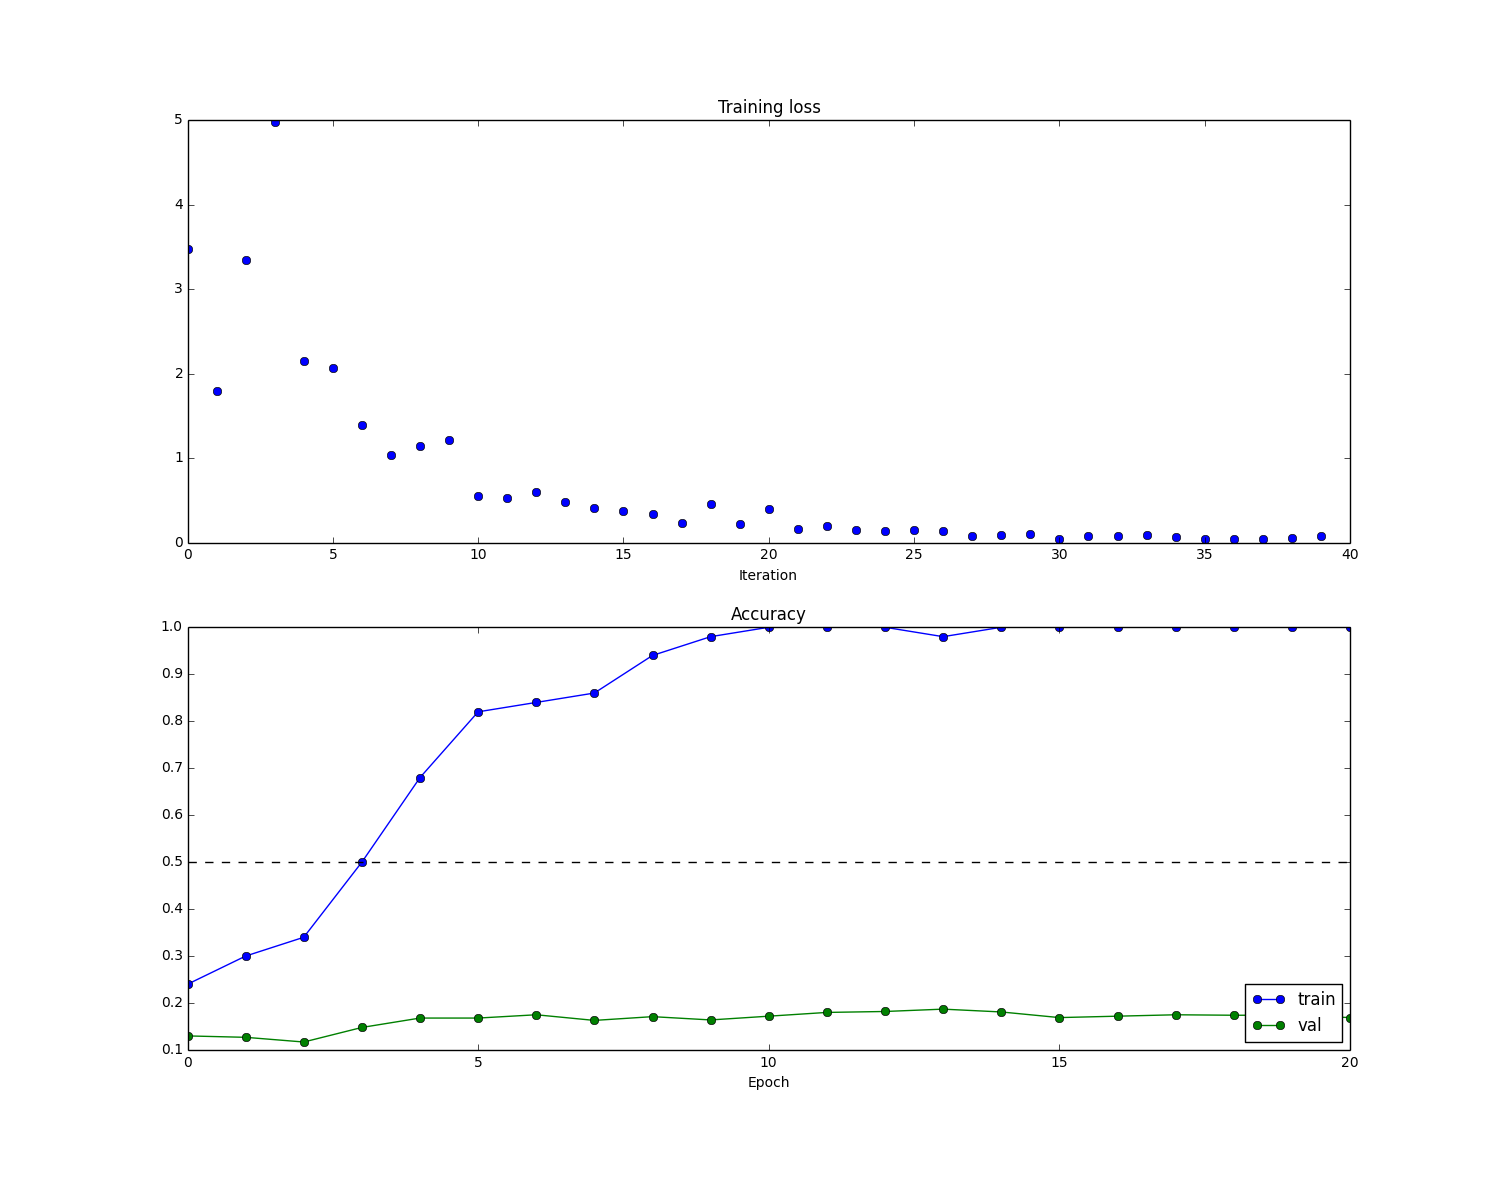
\includegraphics[scale=0.5]{fivetrainingandacc.png}
\end{figure}


Difficulty:
To get an overfitting, deeper network need larger learning rate. Because in the feedback process, we need to transfer a large number, otherwise the first few network will not be trained.
\subsection*{P4.1.10 SGD MOMENTUM}
\begin{lstlisting}
  v = config['momentum'] * v - config['learning_rate'] * dtheta
  next_theta = theta + v
\end{lstlisting}
next\_theta error:  8.88234703351e-09
velocity error:  4.26928774328e-09
\begin{figure}[H]
  \caption{Compare sgd and sgdmomentum}
  \centering
    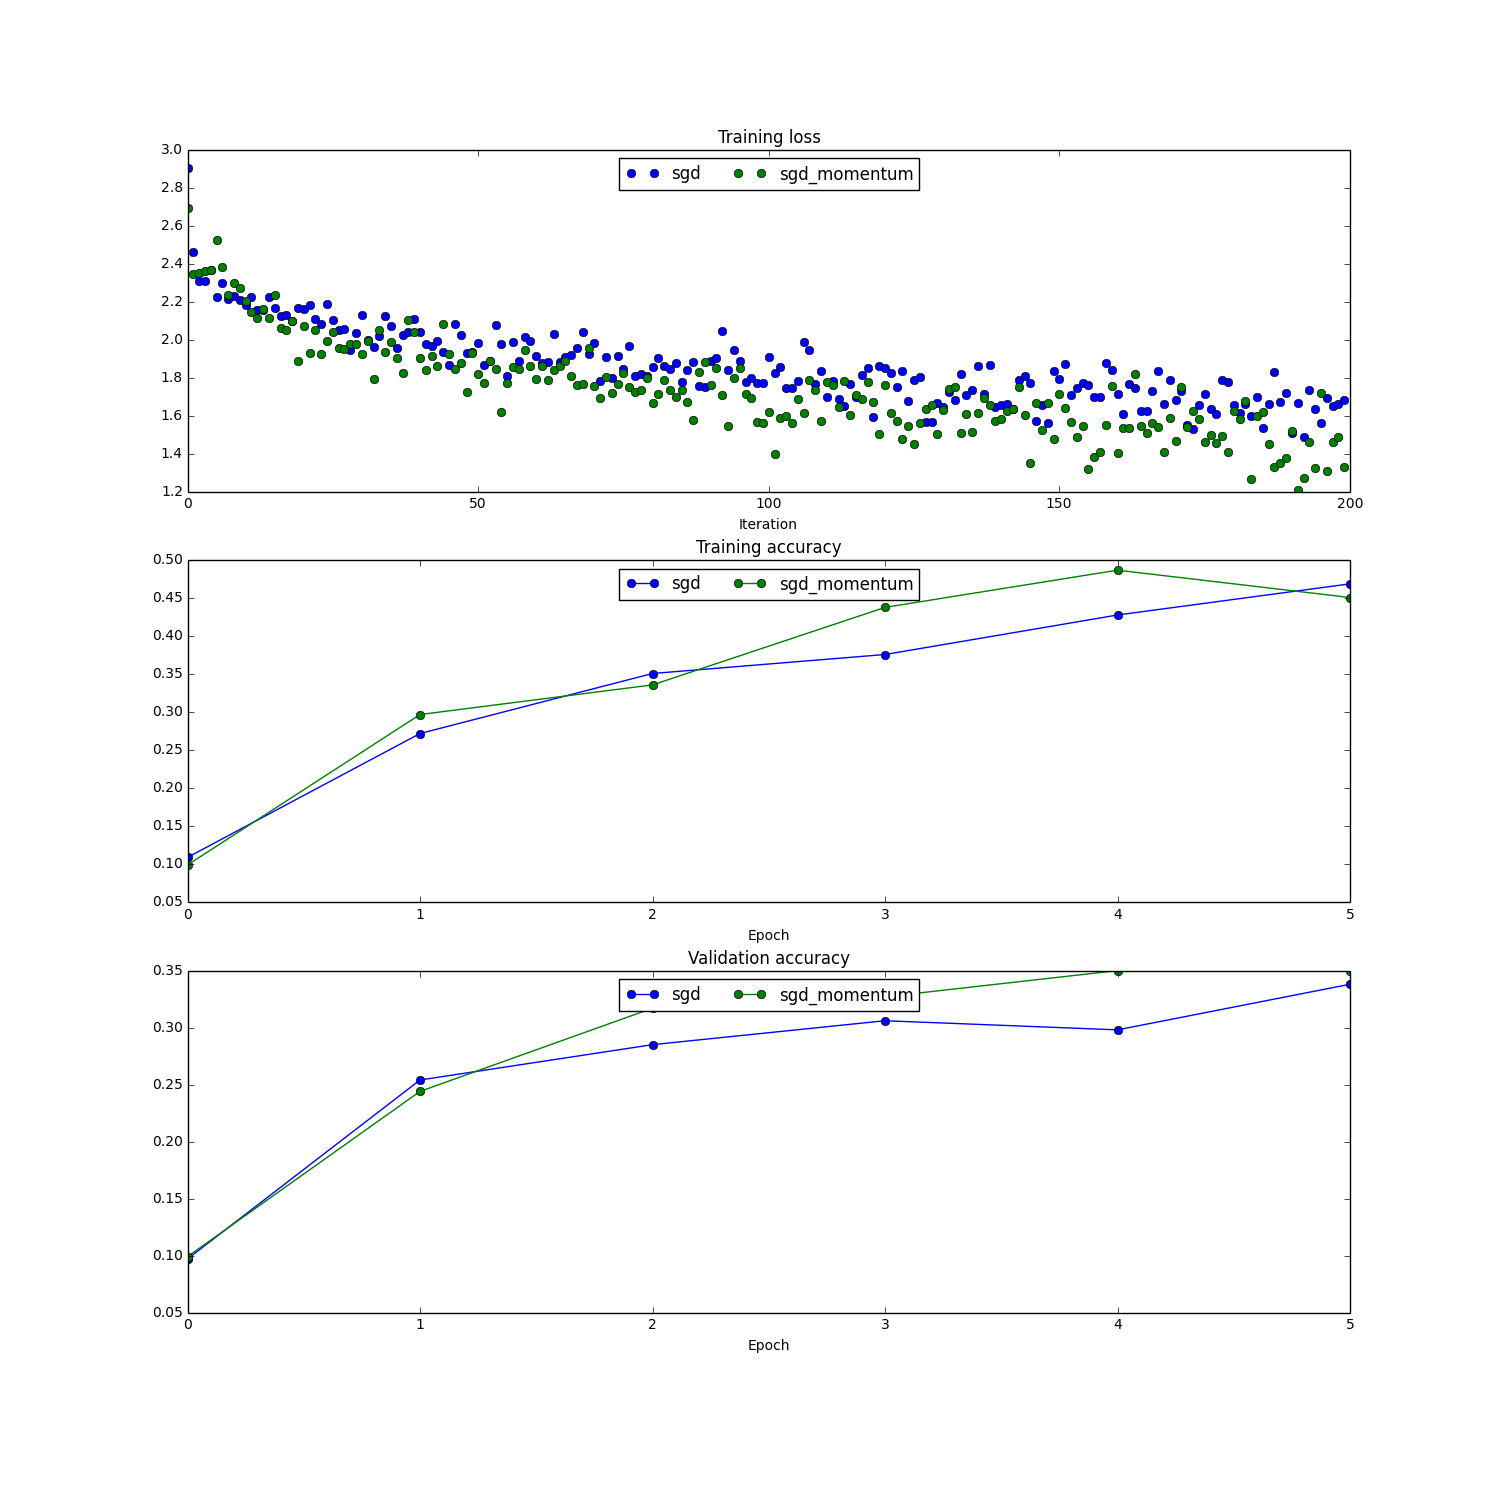
\includegraphics[scale=0.5]{six.png}
\end{figure}


\subsection*{P4.1.11 RMSProp}
\begin{lstlisting}
  config['cache'] = config['decay_rate'] * config['cache'] + \
        (1 - config['decay_rate']) * dtheta ** 2
  next_theta = theta - config['learning_rate'] * \
        dtheta / (np.sqrt(config['cache']) + config['epsilon'])



\end{lstlisting}

next\_theta error:  9.52468751104e-08
cache error:  2.64779558072e-09

\subsection*{P4.1.12 adam}
\begin{lstlisting}
  config['m'] = config['beta1'] * config['m'] + \
        (1 - config['beta1']) * dtheta
  config['v'] = config['beta2'] * config['v'] + \
        (1 - config['beta2']) * (dtheta**2)
  config['t'] += 1

  mt_hat = config['m'] / (1 - (config['beta1'])**config['t'])
  vt_hat = config['v'] / (1 - (config['beta2'])**config['t'])
  next_theta = theta - config['learning_rate'] * \
        mt_hat / (np.sqrt(vt_hat + config['epsilon']))



\end{lstlisting}
next\_theta error:  1.13988746733e-07
v error:  4.20831403811e-09
m error:  4.21496319311e-09
\subsection*{Dropout}

\subsection*{P4.2.1 Dropout forward pass}
\begin{lstlisting}
mask = (np.random.rand(*x.shape) >= p) / (1 - p)
out = x * mask

out = x
\end{lstlisting}
Running tests with p =  0.3
Mean of input:  9.9999440349
Mean of train-time output:  10.0219737942
Mean of test-time output:  9.9999440349
Fraction of train-time output set to zero:  0.298516
Fraction of test-time output set to zero:  0.0

Running tests with p =  0.6
Mean of input:  9.9999440349
Mean of train-time output:  9.94542982254
Mean of test-time output:  9.9999440349
Fraction of train-time output set to zero:  0.602128
Fraction of test-time output set to zero:  0.0

Running tests with p =  0.75
Mean of input:  9.9999440349
Mean of train-time output:  10.0336089444
Mean of test-time output:  9.9999440349
Fraction of train-time output set to zero:  0.749192
Fraction of test-time output set to zero:  0.0


\subsection*{P4.2.2 Dropout backward pass}
\begin{lstlisting}
dx = dout * mask
\end{lstlisting}
dx relative error:  1.89290427118e-11
\subsection*{P4.2.3 Fully connected nets with dropout}




Running check with dropout =  0
Initial loss:  2.3051948274
theta1 relative error: 2.53e-07
theta1\_0 relative error: 2.94e-06
theta2 relative error: 1.50e-05
theta2\_0 relative error: 5.05e-08
theta3 relative error: 2.75e-07
theta3\_0 relative error: 1.17e-10

Running check with dropout =  0.25
Initial loss:  2.30239323056
theta1 relative error: 3.39e-07
theta1\_0 relative error: 3.68e-08
theta2 relative error: 2.24e-07
theta2\_0 relative error: 5.47e-09
theta3 relative error: 1.97e-07
theta3\_0 relative error: 7.54e-11

Running check with dropout =  0.5
Initial loss:  2.30134643809
theta1 relative error: 1.29e-07
theta1\_0 relative error: 6.99e-09
theta2 relative error: 3.95e-07
theta2\_0 relative error: 2.82e-09
theta3 relative error: 4.28e-07
theta3\_0 relative error: 8.93e-11




\subsection*{P4.2.4 Fully connected nets with dropout}

when the dropout=0, we finally get train acc: 0.998000; val\_acc: 0.302000\\
when the dropout=0.75, we get train acc: 1.000000; val\_acc: 0.313000.
\begin{figure}[H]
  \caption{compare dropout}
  \centering
    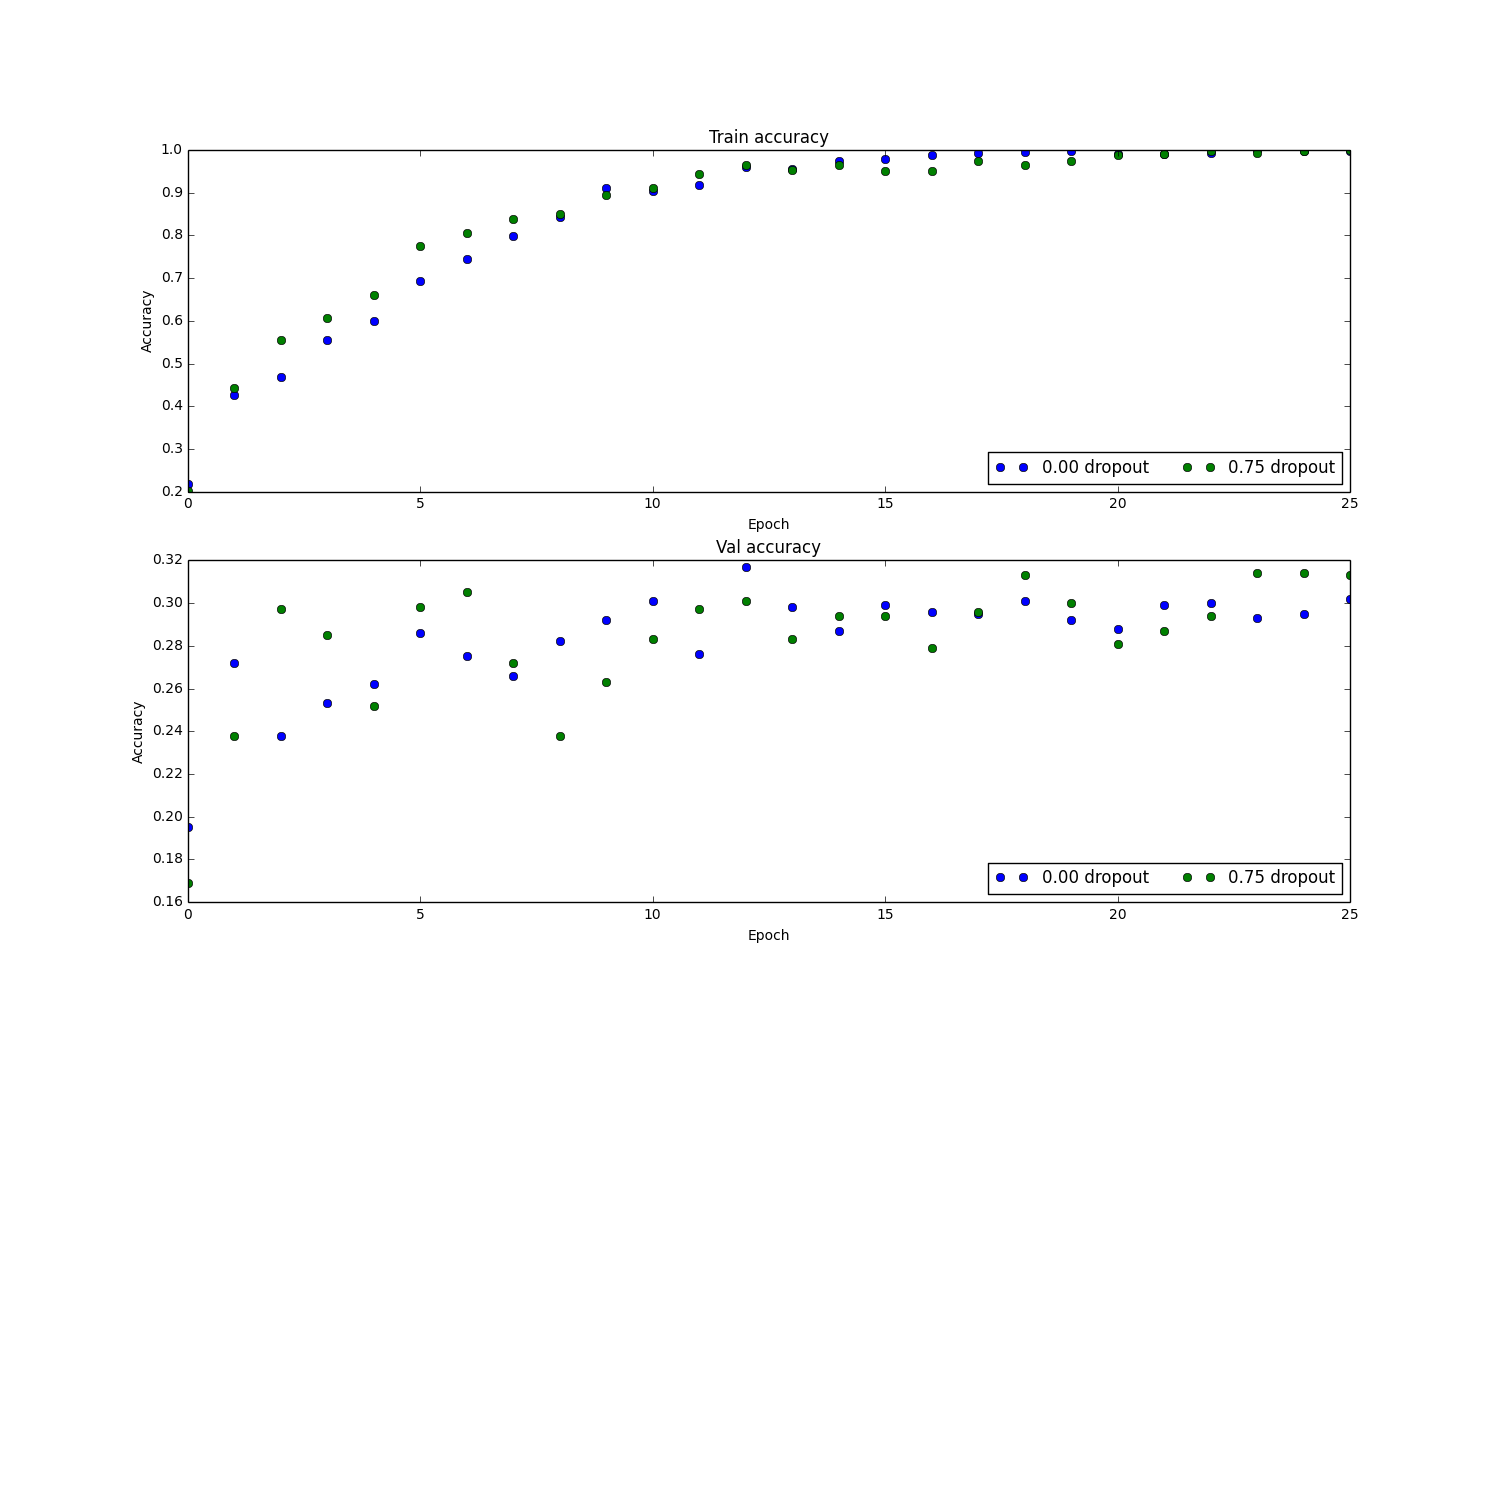
\includegraphics[scale=0.5]{dropout.png}
\end{figure}

Comment:
On training set, two networks all go to converge, the slope of accuracy all go down with increasing epoch.
The network with dropout converge faster with dropout in the training data. In validation data, with or without dropout, the networks all have similar fluctuation. Generally speaking, the network with dropout has higher accuracy in validation set.

\section*{P4.3 train a fully connected net for the cifar-10 with dropout}
\begin{lstlisting}
% * <xun6000@gmail.com> 2017-03-26T04:00:51.675Z:
%
% ^.
% * <xun6000@gmail.com> 2017-03-26T04:00:50.101Z:
%
% ^.


best_model = None

best_model = FullyConnectedNet([100, 200, 100,100,100,100], weight_scale=5e-2,dropout=0.75) # input size, hidden size, number of classes 
solver = Solver(best_model, data, num_epochs=18, batch_size=100, update_rule=update_rule, 
                optim_config={ 'learning_rate': 2.5e-3 }, verbose=True)  #47 100,200,100 2.5 10 ci duiying 4ceng 

solver.train()


\end{lstlisting}
finally we get accuracy 
(Epoch 18 / 18) train acc: 0.673000; val\_acc: 0.509000
\subsection*{Test model}
\begin{lstlisting}
from vis_utils import visualize_grid
X_test=data['X_test']
y_test=data['y_test']
X_val=data['X_val']
y_val=data['y_val']
def show_net_weights(net):
  W1 = net.params['theta1']
  W1 = W1.reshape(32, 32, 3, -1).transpose(3, 0, 1, 2)
  plt.imshow(visualize_grid(W1, padding=3).astype('uint8'))
  plt.gca().axis('off')
  #plt.show()
  plt.savefig("visual.png")


show_net_weights(best_model)
y_test_pred = np.argmax(best_model.loss(X_test), axis=1)
y_val_pred = np.argmax(best_model.loss(X_val), axis=1)
print 'Validation set accuracy: ', (y_val_pred == y_val).mean()
print 'Test set accuracy: ', (y_test_pred == y_test).mean()
\end{lstlisting}

Validation set accuracy:  0.512
Test set accuracy:  0.496

\begin{figure}[H]
  \caption{Visualize the weight}
  \centering
    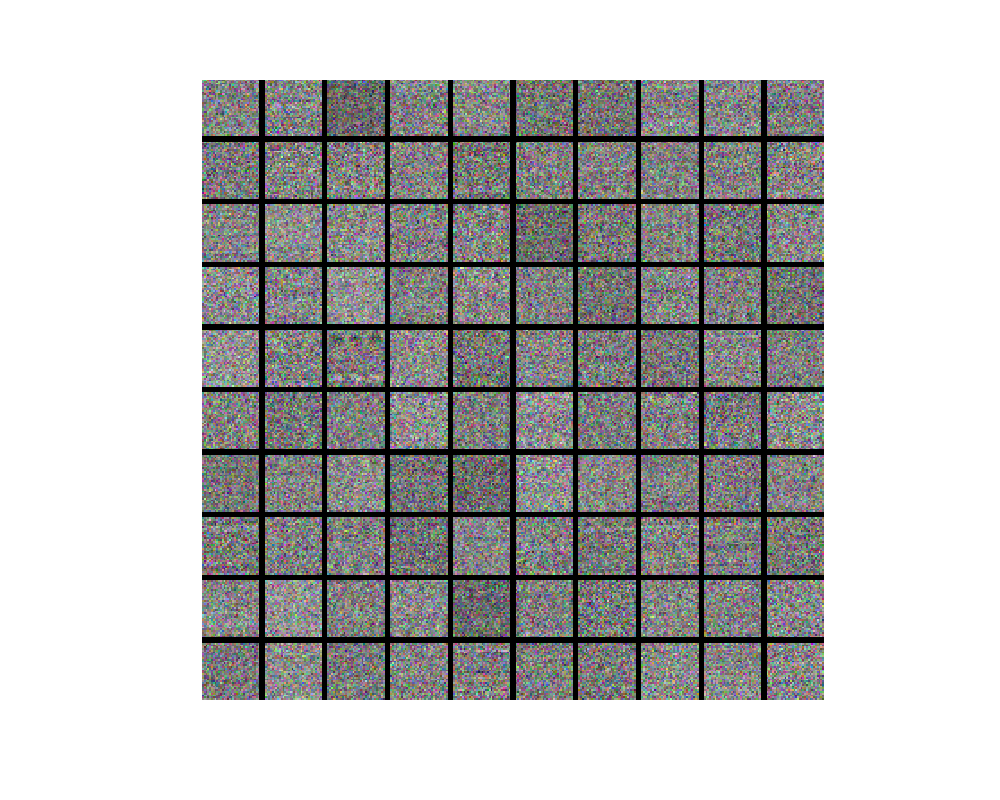
\includegraphics[scale=0.5]{visual.png}
\end{figure}


\subsection*{Prob 4.4.1 CNN forward pass}

\begin{lstlisting}
M, C, H, W = x.shape
  K, C, HH, WW = theta.shape
  pad, stride = conv_param['pad'], conv_param['stride']
  H_ = int(1 + (H + 2. * pad - HH) / stride)
  W_ = int(1 + (W + 2. * pad - WW) / stride)
  out = np.zeros([M, K, H_, W_])
  X = np.pad(x, ((0, 0), (0, 0), (pad, pad), (pad, pad)), 'constant')

  for k in xrange(K):
      theta_ = theta[k].reshape(C * HH * WW)
      for m in xrange(M):
          for h in xrange(0, H, stride):
              for w in xrange(0, W, stride):
                  x_ = X[m, :, h:h + HH, w:w + WW].reshape(C * HH * WW)
                  out[m, k, h / stride, w / stride] = theta_.dot(x_.T) + theta0[k]
  
\end{lstlisting}
Here is the result:
Testing conv\_forward\_naive
difference:  2.21214764175e-08
\begin{figure}[H]
  \caption{compare dropout}
  \centering
    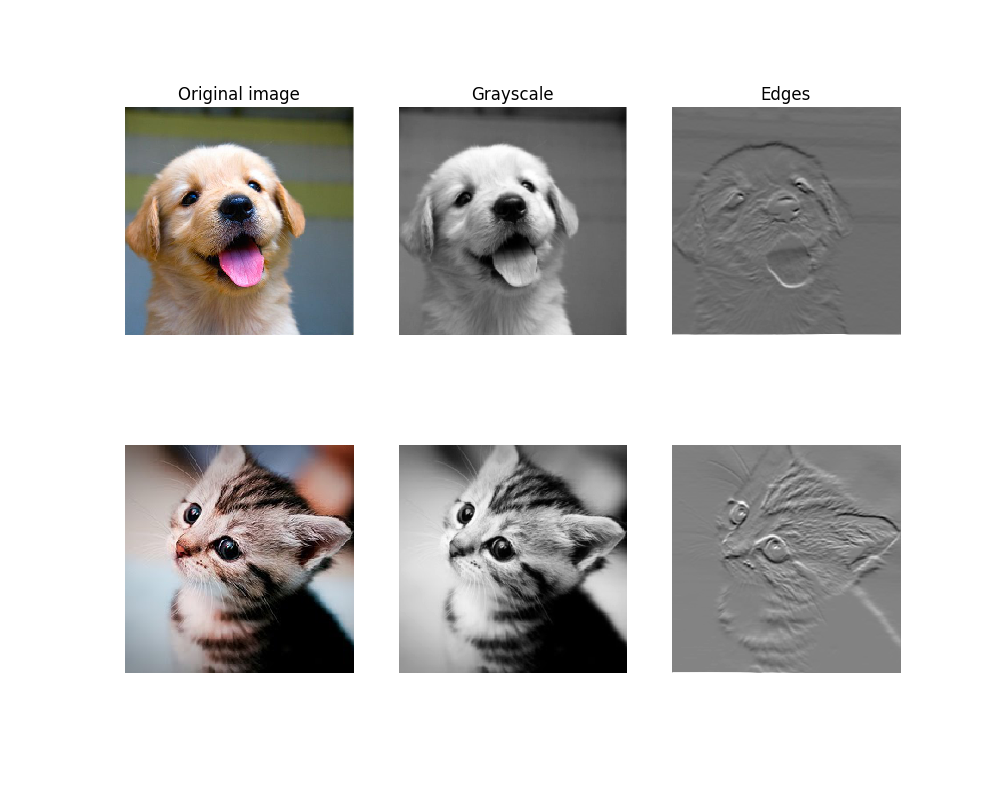
\includegraphics[scale=0.5]{dog.png}
\end{figure}


\subsection*{Prob 4.4.2 CNN backward pass}

\begin{lstlisting}
  x, theta, theta0, conv_param = cache
  M, C, H, W = x.shape
  K, C, HH, WW = theta.shape
  M, K, H_, W_ = dout.shape
  P, S = conv_param['pad'], conv_param['stride']
  X = np.pad(x, ((0, 0), (0, 0), (P, P), (P, P)), 'constant')
  dx, dtheta, dtheta0 = np.zeros_like(X), np.zeros_like(theta), np.zeros_like(theta0)

  for k in xrange(K):
      theta_ = theta[k]
      for m in xrange(M):
          for h in xrange(0, H, S):
              for w in xrange(0, W, S):
                  x_ = X[m, :, h:h + HH, w:w + WW]
                  dout_ = dout[m, k, h / S, w / S]
                  dtheta0[k] += dout_
                  for hh in xrange(HH):
                      for ww in xrange(WW):
                          dx[m, :, h + hh, w + ww] += dout_ * theta_[:, hh, ww]
                          dtheta[k, :, hh, ww] += dout_ * x_[:, hh, ww]
  dx = dx[:, :, 1:-1, 1:-1]

\end{lstlisting}
Here is the result:
Testing conv\_backward\_naive function
dx error:  9.24931044013e-09
dtheta error:  8.96365265076e-09
dtheta0 error:  2.02901864605e-11





\subsection*{Prob 4.4.3 max pooling forward}

\begin{lstlisting}
M, C, H, W = x.shape
  Fh, Fw, S = pool_param['pool_height'], pool_param['pool_width'], pool_param['stride']
  H2 = int(1 + (H - Fh) / S)
  W2 = int(1 + (W - Fw) / S)
  out = np.zeros([M, C, H2, W2])

  for m in xrange(M):
      for h in xrange(0, H, S):
          for w in xrange(0, W, S):
              for c in xrange(C):
                  out[m, c, h / S, w / S] = np.max(x[m, c, h:h + Fh, w:w + Fw])
    
 
\end{lstlisting}

Testing max\_pool\_forward\_naive function:
difference:  4.16666651573e-08
\subsection*{Prob 4.4.4 max pooling backward}

\begin{lstlisting}
x, pool_param = cache
  M, C, H, W = x.shape
  Fh, Fw, S = pool_param['pool_height'], pool_param['pool_width'], pool_param['stride']
  M, C, H2, W2 = dout.shape
  dx = np.zeros_like(x)

  for m in xrange(M):
      for h in xrange(0, H, S):
          for w in xrange(0, W, S):
              for c in xrange(C):
                  maxh, maxw = np.unravel_index(np.argmax(x[m, c, h:h + Fh, w:w + Fw]), [Fh, Fw])
                  dx[m, c, h + maxh, w + maxw] = dout[m, c, h / S, w / S]
    
  
\end{lstlisting}
Testing max\_pool\_backward\_naive function:
dx error:  3.27561689344e-12







\subsection*{fast layer}
\begin{lstlisting}
Testing conv_forward_fast:
Naive: 2.821562s
Fast: 0.021149s
Speedup: 133.414001x
Difference:  1.15755875767e-11

Testing conv_backward_fast:
Naive: 42.759402s
Fast: 0.020618s
Speedup: 2073.890828x
dx difference:  7.11628676988e-12
dw difference:  1.96607042014e-12
db difference:  2.67913473524e-14

Testing pool_forward_fast:
Naive: 0.453308s
fast: 0.005545s
speedup: 81.748689x
difference:  0.0

Testing pool_backward_fast:
Naive: 0.570289s
speedup: 30.953543x
dx difference:  0.0
  
\end{lstlisting}

\subsection*{sandwish layer}

\begin{lstlisting}
Testing conv_relu_pool
dx error:  3.35592723922e-08
dtheta error:  7.82678129546e-10
dtheta0 error:  2.99441544456e-11
  
\end{lstlisting}


\begin{lstlisting}
Testing conv_relu:
dx error:  5.22188261691e-09
dtheta error:  1.06772812654e-09
dtheta0 error:  1.34962661485e-11
  
\end{lstlisting}


\subsection*{Three layer cnn}
\begin{lstlisting}
    self.params['theta1'] = np.random.randn(
            num_filters, input_dim[0], filter_size, filter_size) * weight_scale
    self.params['theta1_0'] = np.zeros((num_filters,))
    self.params['theta2'] = np.random.randn(
            num_filters * input_dim[1] * input_dim[2] / 4, hidden_dim) * weight_scale
    self.params['theta2_0'] = np.zeros((hidden_dim,))
    self.params['theta3'] = np.random.randn(
            hidden_dim, num_classes) * weight_scale
    self.params['theta3_0'] = np.zeros((num_classes,))
  
\end{lstlisting}

\begin{lstlisting}

    out1, cache1 = conv_relu_pool_forward(X, theta1, theta1_0, conv_param, pool_param)
    out2, cache2 = affine_relu_forward(out1, theta2, theta2_0)
    scores, cache3 = affine_forward(out2, theta3, theta3_0)
  
\end{lstlisting}
\begin{lstlisting}

    loss, dxl = softmax_loss(scores, y)
    loss += self.reg / 2. * (np.sum(theta1 ** 2) +
                                 np.sum(theta2 ** 2) +
                                 np.sum(theta3 ** 2))

    dx3, dtheta3, dtheta_03 = affine_backward(dxl, cache3)
    grads['theta3'] = dtheta3 + self.reg * theta3
    grads['theta3_0'] = dtheta_03

    dx2, dtheta2, dtheta_02 = affine_relu_backward(dx3, cache2)
    grads['theta2'] = dtheta2 + self.reg * theta2
    grads['theta2_0'] = dtheta_02

    dx, dtheta, dtheta_01 = conv_relu_pool_backward(dx2, cache1)
    grads['theta1'] = dtheta + self.reg * theta1
    grads['theta1_0'] = dtheta_01
\end{lstlisting}

\subsection*{loss}

\begin{lstlisting}
Initial loss (no regularization):  2.30258756632
Initial loss (with regularization):  2.50886715705
\end{lstlisting}

\subsection*{gradient}

\begin{lstlisting}
theta1 max relative error: 1.003907e-01
theta1_0 max relative error: 8.626337e-02
theta2 max relative error: 2.219676e-02
theta2_0 max relative error: 2.397835e-06
theta3 max relative error: 1.700603e-05
theta3_0 max relative error: 1.281512e-09
\end{lstlisting}
\subsection*{Overfit small data}
\begin{lstlisting}
Here is the result:
(Iteration 40 / 40) loss: 0.011704
(Iteration 40 / 40) loss: 0.015240
(Epoch 20 / 20) train acc: 1.000000; val_acc: 0.218000
\end{lstlisting}
\begin{figure}[H]
  \caption{loss and accuracy of small data}
  \centering
    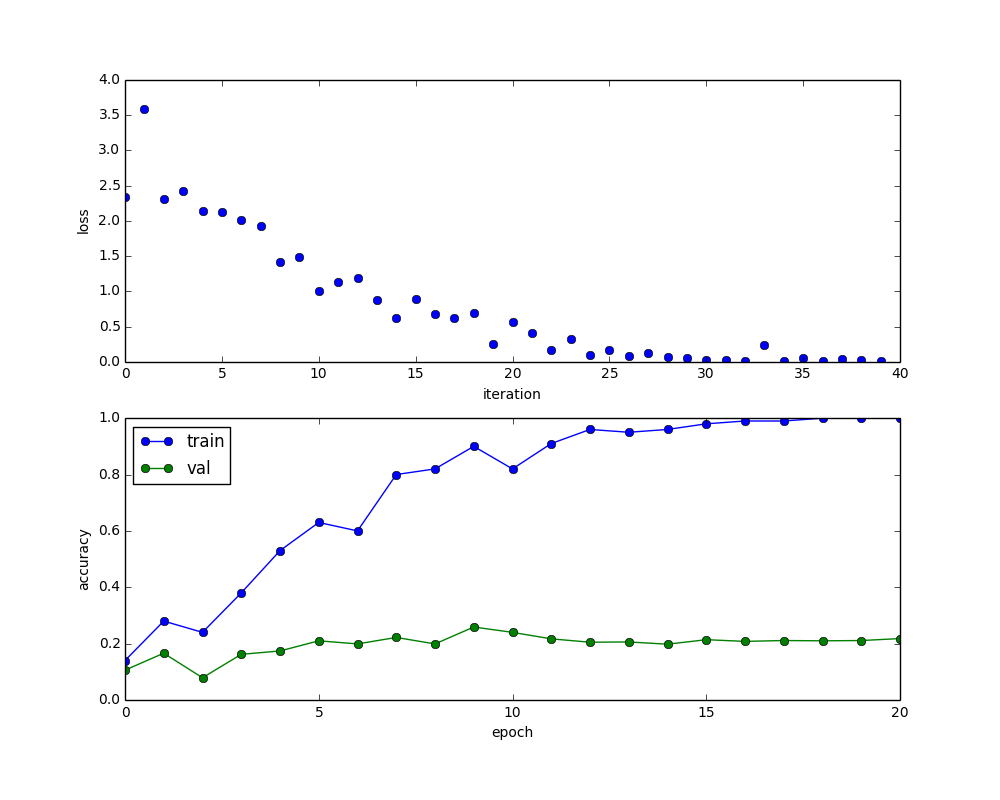
\includegraphics[scale=0.5]{smalldata.png}
\end{figure}


\subsection*{train the nect on cifer data}
Here is the result
\begin{lstlisting}
(Iteration 961 / 980) loss: 1.764696
(Epoch 1 / 1) train acc: 0.486000; val_acc: 0.484000
\end{lstlisting}





\begin{figure}[H]
  \caption{filter}
  \centering
    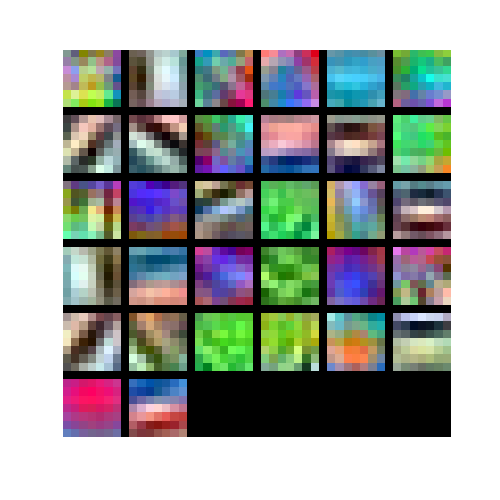
\includegraphics[scale=0.5]{filter.png}
\end{figure}

\subsection*{extra}
Here is our result:
\begin{lstlisting}
(Iteration 9781 / 9800) loss: 0.170941
(Epoch 10 / 10) train acc: 0.926000; val_acc: 0.655000
\end{lstlisting}
The code is in the python file.
we finally get test accuracy of 0.67.
\begin{figure}[H]
  \caption{my best model}
  \centering
    \includegraphics[scale=0.5]{extra.png}
\end{figure}
Other stuff are in the ipynb file.






\end{document}

